%! TEX root = ../../main.tex

\subsection{Design Science Research}%
\label{sub:Design_Science_Research}

When designing the optimal information system that is able to continuously
deploy microservices, the obvious outcome is a practical model. This model is
embedded in some technical environment but may not contribute any scientific
findings. That is the reason why this thesis uses the \ac{DSR} approach for
designing information systems. \ac{DSR} is an conceptual framework that can be
applied to any research project. It defines seven principal guidelines that
govern the way research should be conducted. This section will explore the
workings of \ac{DSR} and how it will be utilised in this research endeavour.

In general, the goal behind \ac{DSR} is to design \ac{IT} \textit{artefacts}.
An artefact can not only be an instantiation, e.g.\ a software prototype, but
can also be a construct, model and method that is utilised in the development
and usage of information systems \autocite[p.
82]{VonAlanDesignscienceinformation2004}.

The creation of artefacts is regulated by seven guidelines. These guidelines
assure that the requirements for the conducted research are apprehensible for
both the researcher as well as the reader \autocite[p.
82]{VonAlanDesignscienceinformation2004}.

\LTXtable{\textwidth}{tables/design_science.tex}

Table~\ref{tab:design_science_guidelines} lists these guidelines. The intensity
to which the guidelines are enforced can be varied according to the respective
research project. However every guideline should be addressed in some form
\autocite[p.  82]{VonAlanDesignscienceinformation2004}. 

\ac{DSR} also defines a fundamental development cycle. Figure
~\ref{fig:design_science_cycles} shows this cycle embedded inside the \ac{DSR}
\textit{components}. The environment component provides the context, e.g.\ the
research question, for any given research. It consists of all entities acting
inside of the environment. All designed artefacts have to be tested inside the
environment in order to assure that they really solve the identified problem
\autocite[p. 89]{HevnerThreeCycleView2007}.

\begin{figure}[H]
\begin{center}
  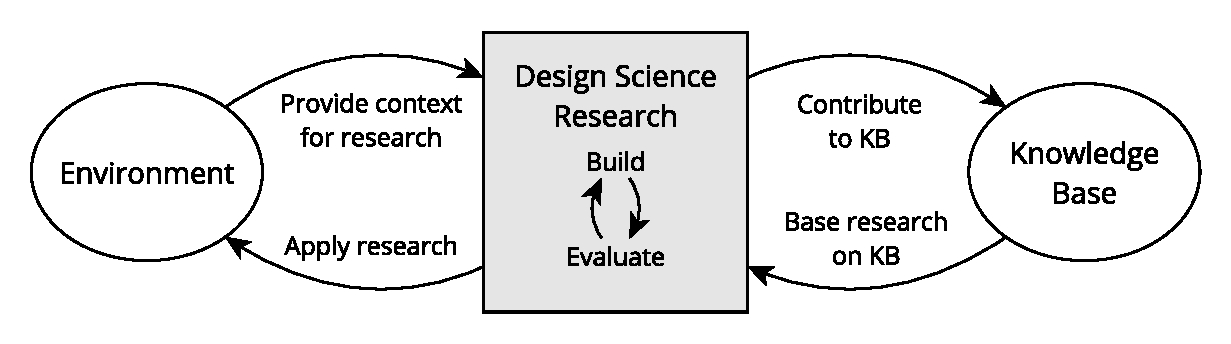
\includegraphics[scale=0.7]{images/figures/design_science_cycles.pdf}
\end{center}
\caption[Simplified interaction model between the environment, knowledge base and Design Science Research.]{Simplified interaction model between the environment, knowledge base and Design Science Research (adapted from \autocite[Fig. 1]{HevnerThreeCycleView2007}).}
\label{fig:design_science_cycles}
\end{figure}

When building artefacts, guideline seven states that any research has to be
conducted rigorously. To achieve this, theoretical foundations as well as
methodologies from the knowledge base can be used \autocite[p.
88]{VonAlanDesignscienceinformation2004}. After an artefact is fully designed,
the findings have to be contributed to the knowledge base; either in the form
of the artefact itself, foundations or methodologies.

The actual development cycle consists of building an artefact and evaluating it
iteratively. Each time this cycle is executed the artefact improves. Such an
evaluation can e.g.\ be performed in an experiment \autocite[p.
91]{HevnerThreeCycleView2007}.

In most cases, an artefact does not represent a complete information system. It
much more tries to capture the ideas, methods and processes that are needed to
design and use an information system \autocite[p.
83]{VonAlanDesignscienceinformation2004}.

In this thesis, for each \href{link:problem_domains}{problem domain} at least
one artefact will be developed. These artefacts answer the research question of
their respective problem domain. 

% TODO: Details zur Verwendung von DSR hinzufügen
